%%%%%%%%%%%%%%%%%%%%%%%%%%%%%%%%%%%%%%%%%
% Beamer Presentation
% LaTeX Template
% Version 1.0 (10/11/12)
%
% This template has been downloaded from:
% http://www.LaTeXTemplates.com
%
% License:
% CC BY-NC-SA 3.0 (http://creativecommons.org/licenses/by-nc-sa/3.0/)
%
%%%%%%%%%%%%%%%%%%%%%%%%%%%%%%%%%%%%%%%%%

%----------------------------------------------------------------------------------------
%	PACKAGES AND THEMES
%----------------------------------------------------------------------------------------

\documentclass{beamer}

\mode<presentation> {

% The Beamer class comes with a number of default slide themes
% which change the colors and layouts of slides. Below this is a list
% of all the themes, uncomment each in turn to see what they look like.

%\usetheme{default}
%\usetheme{AnnArbor}
%\usetheme{Antibes}
%\usetheme{Bergen}
%\usetheme{Berkeley}
%\usetheme{Berlin}
%\usetheme{Boadilla}
%\usetheme{CambridgeUS}
%\usetheme{Copenhagen}
%\usetheme{Darmstadt}
%\usetheme{Dresden}
%\usetheme{Frankfurt}
%\usetheme{Goettingen}
%\usetheme{Hannover}
%\usetheme{Ilmenau}
%\usetheme{JuanLesPins}
%\usetheme{Luebeck}
\usetheme{Madrid}
%\usetheme{Malmoe}
%\usetheme{Marburg}
%\usetheme{Montpellier}
%\usetheme{PaloAlto}
%\usetheme{Pittsburgh}
%\usetheme{Rochester}
%\usetheme{Singapore}
%\usetheme{Szeged}
%\usetheme{Warsaw}

% As well as themes, the Beamer class has a number of color themes
% for any slide theme. Uncomment each of these in turn to see how it
% changes the colors of your current slide theme.

%\usecolortheme{albatross}
%\usecolortheme{beaver}
%\usecolortheme{beetle}
%\usecolortheme{crane}
%\usecolortheme{dolphin}
%\usecolortheme{dove}
%\usecolortheme{fly}
%\usecolortheme{lily}
%\usecolortheme{orchid}
%\usecolortheme{rose}
%\usecolortheme{seagull}
%\usecolortheme{seahorse}
%\usecolortheme{whale}
%\usecolortheme{wolverine}

%\setbeamertemplate{footline} % To remove the footer line in all slides uncomment this line
%\setbeamertemplate{footline}[page number] % To replace the footer line in all slides with a simple slide count uncomment this line

%\setbeamertemplate{navigation symbols}{} % To remove the navigation symbols from the bottom of all slides uncomment this line
}

\usepackage{graphicx} % Allows including images
\usepackage{booktabs} % Allows the use of \toprule, \midrule and \bottomrule in tables

%----------------------------------------------------------------------------------------
%	TITLE PAGE
%----------------------------------------------------------------------------------------

\title[Desgin pattern Fly Weight]{Desgin patterns: Fly weight, an optimised desgin} % The short title appears at the bottom of every slide, the full title is only on the title page

\author{Arthur REMOND et Tigran SLAMA} % Your name
\institute[ULCO] % Your institution as it will appear on the bottom of every slide, may be shorthand to save space
{
Universite du Littoral Cote d'Opale \\ % Your institution for the title page
\medskip
\textit{} % Your email address
}
\date{\today} % Date, can be changed to a custom date

\begin{document}

\begin{frame}
\titlepage % Print the title page as the first slide
\end{frame}

\begin{frame}
 \tableofcontents
\end{frame}

\begin{frame}{Fly Weight Pattern}
    \begin{center}
        \includegraphics[scale=0.5]{comics.png}
    \end{center}
\end{frame}

%----------------------------------------------------------------------------------------
%	PRESENTATION SLIDES
%----------------------------------------------------------------------------------------

%------------------------------------------------
\section{Fly Weight}
%------------------------------------------------

\subsection{Fly Weight}
\begin{frame}
\frametitle{Fly Weight}
\begin{block}{Catégorie}
Pattern structurel: permet d'assembler objets et des classes dans des structures larges tout en conservant ces structures flexibles et maintenables.
\end{block}
\begin{block}{Problématique}
Comment gérer efficacement dans la mémoire l'accumulation d'objets ayant des attributs identiques ? Réduire l'empreinte de ce genre de système en RAM ?
\end{block}

\end{frame}

% -----
\subsection{État intrinsèque et extrinsèque}

\begin{frame}
\frametitle{État intrinsèque et extrinsèque}

\begin{itemize}

    \item Intrinsèque
        \begin{itemize}
            \item Nom
            \item Vie
        \end{itemize}

    \item
        \begin{minipage}[c]{0.5\linewidth}
        Extrinsèque: Arme
        \end{minipage}
        \begin{minipage}[c]{0.3\linewidth}
        \centering
        \strut\vspace*{-\baselineskip}\newline\includegraphics[scale=0.2]{flywright_character.png}
        \end{minipage}

\end{itemize}
\end{frame}

%------------------------------------------------
\begin{frame}
\frametitle{Fly Weight}

    \begin{block}{Objectif}
    Partager les similitudes d'états entre plusieurs objets afin de réduire l'empreinte mémoire.
    \end{block}

    \begin{block}{Intérêt}
    \begin{itemize}
    \item Gestion d'objets en RAM
    \item Partage d'instances
    \item Extraire un état complexe dans plusieurs états immuables partagés.
    \end{itemize}
    \end{block}
\end{frame}

%------------------------------------------------

\subsection{Fly Weight Factory}
\begin{frame}
\frametitle{Fly Weight Factory}
Le pattern Fly Weight s'utilise naturellement avec le pattern Factory *.

\begin{block}{* Pattern Factory}
Pattern permettant la création d'objets derrière une interface.
\end{block}

\end{frame}

%------------------------------------------------
\section{Real world analogy}
%------------------------------------------------

\subsection{Exemple: Simulateur de véhicules}

\begin{frame}
\frametitle{Real world example}

Jeux vidéo:
\begin{itemize}
\item Effets de particules dans les animations
\item Costumes / Accessoires des personnages
\item Une forêt de plusieurs types d'arbres
\end{itemize}
\end{frame}

%------------------------------------------------

\begin{frame}
\frametitle{Exemple: Simulateur de véhicules}
\begin{block}{Exemple}
Nous souhaitons réaliser un simulateur de véhicules dans une ville avec des voitures, des camions, des vélos etc.
Nous voudrions pouvoir observer la solution dans une carte interactive.
La solution doit pouvoir envisager l'amélioration avec d'autres types de véhicules.
\end{block}
\end{frame}

%------------------------------------------------

\begin{frame}
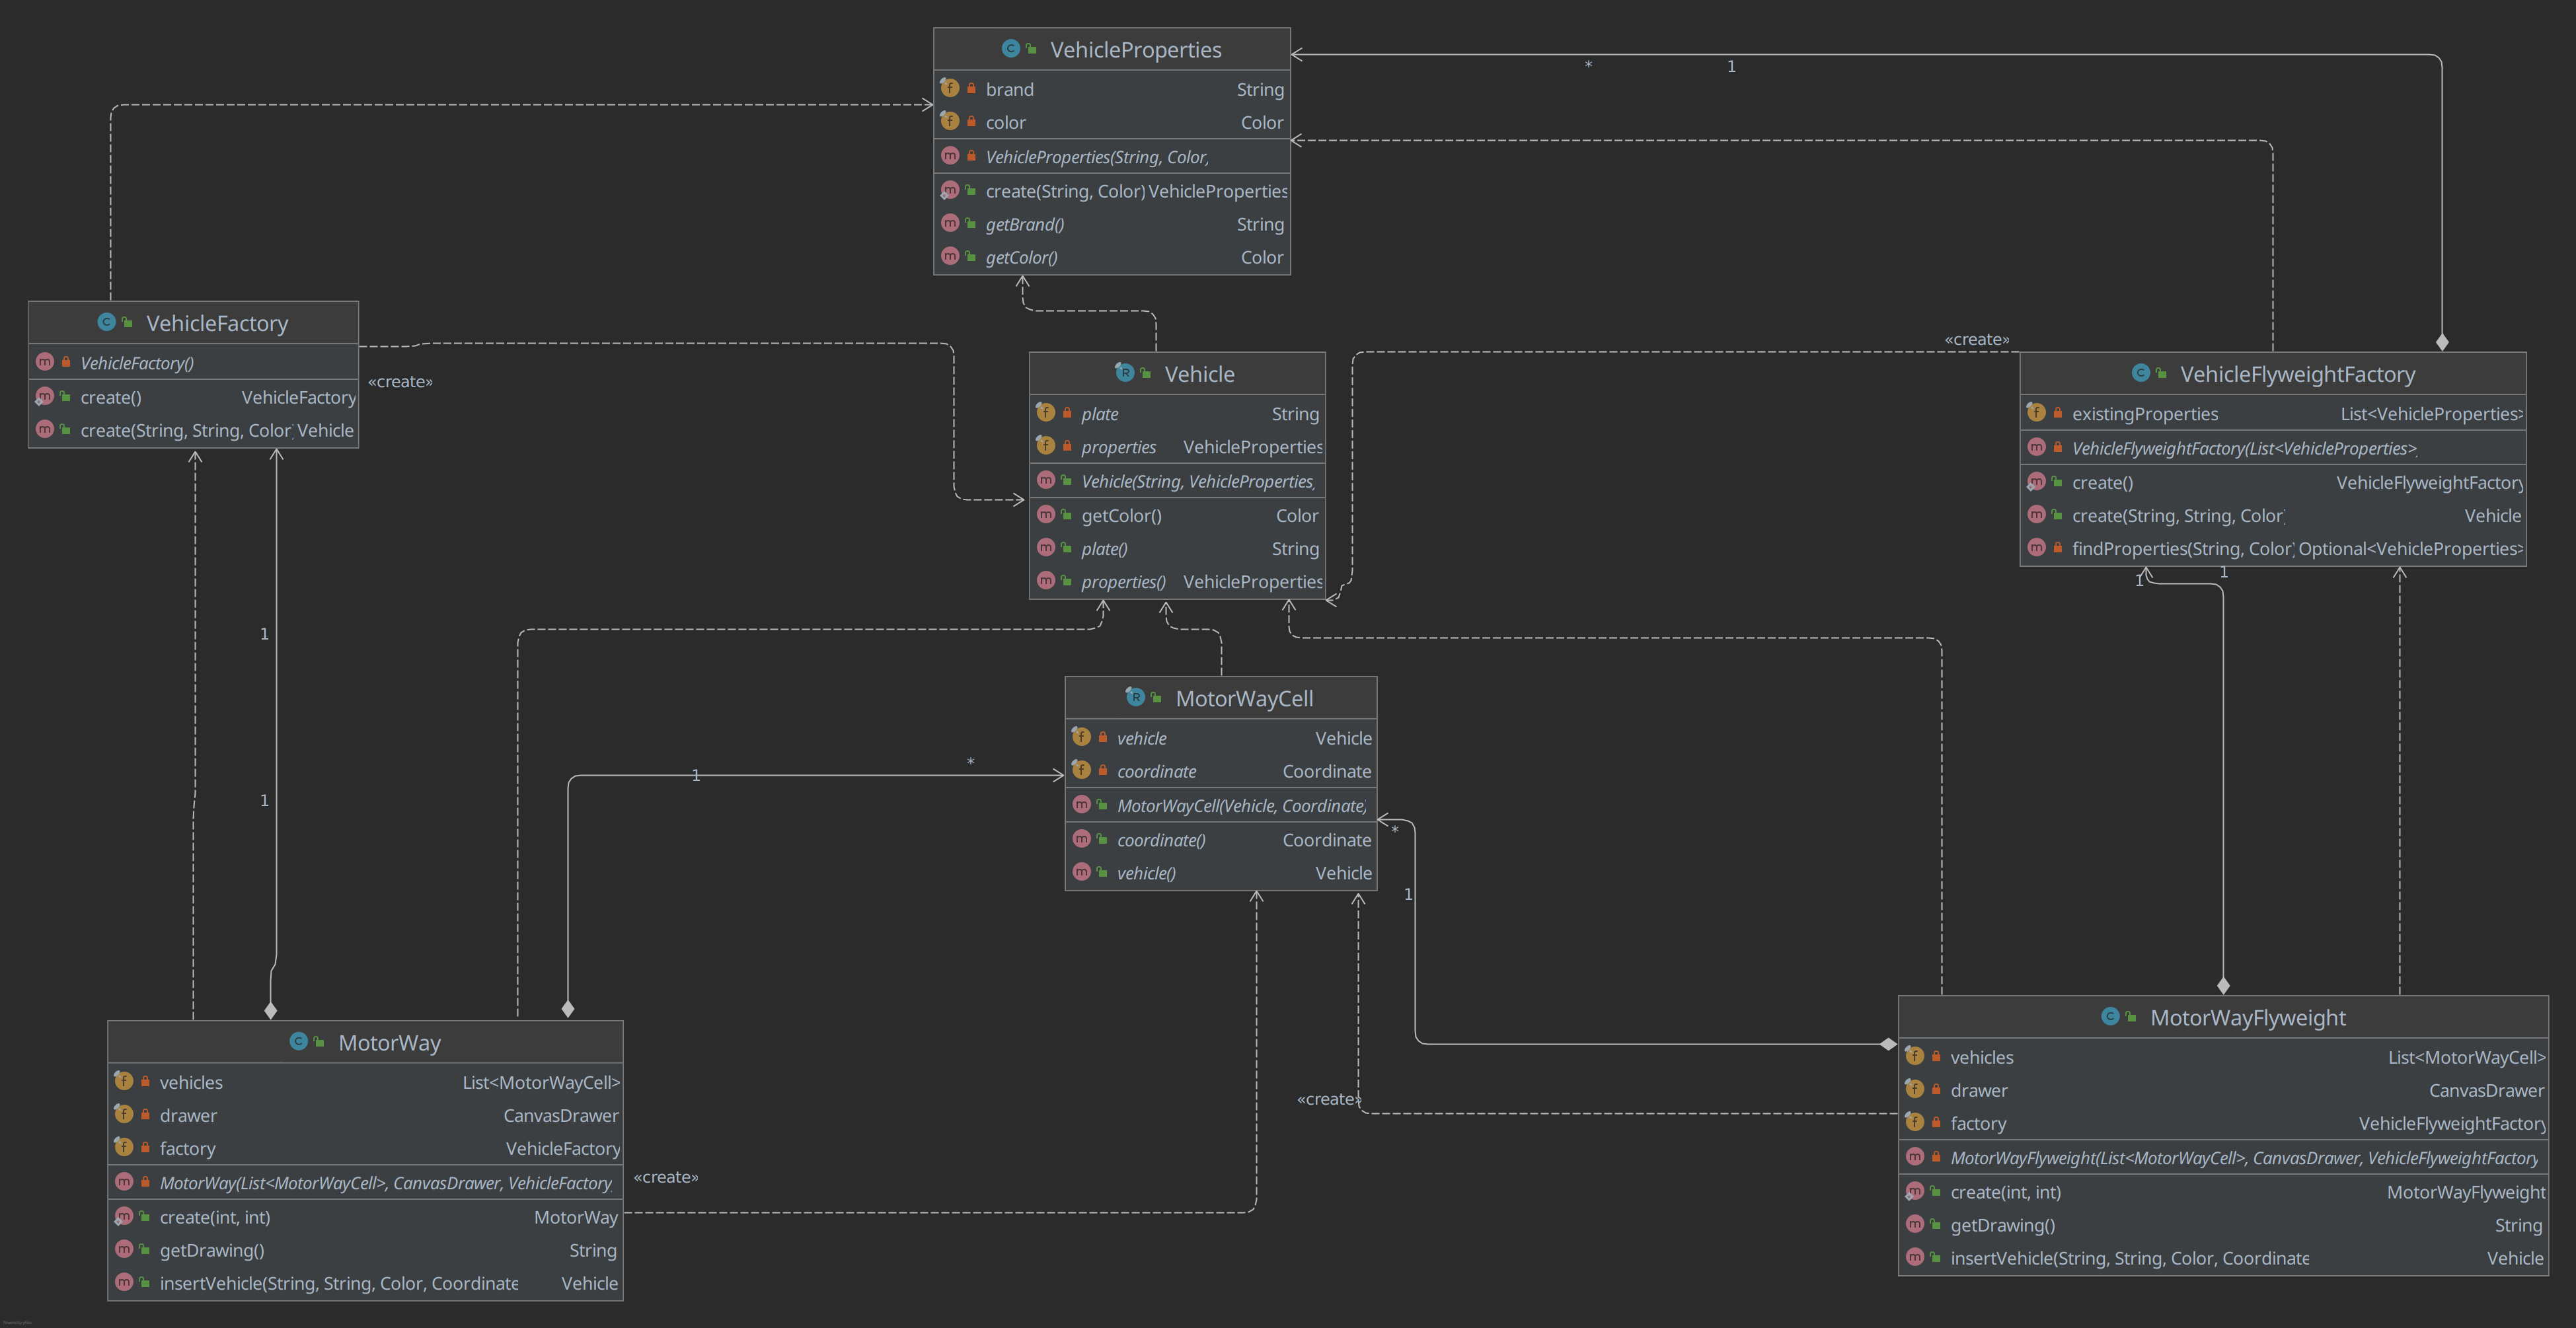
\includegraphics[scale=0.09]{FlyWeightFactories.png}
\end{frame}

%------------------------------------------------

\subsection{Quelques comparaisons}

\begin{frame}
\frametitle{Quelques comparaisons}

\begin{block}{}
Pour 10 000 000 de véhicules avec 10 propriétés différentes:

\begin{itemize}
    \item Normal: 1130.46875 mo
    \item FlyWeight: 277.46875 mo
\end{itemize}

\end{block}
\end{frame}

%------------------------------------------------

\begin{frame}
\frametitle{Quelques comparaisons}

\begin{center}
    \includegraphics[scale=0.5]{flyweightres.png}
\end{center}
    Évolution du temps de création pour X objets (Intel i5\-7300HQ (4) \@ 3.500GHz)

\end{frame}

%------------------------------------------------

\subsection{Avantages et Inconvénients}

\begin{frame}
\frametitle{Avantages et Inconvénients}

\begin{block}{Avantages}

\begin{itemize}
\item Permet d'économiser beaucoup de RAM
\end{itemize}
\end{block}

\begin{block}{Inconvénients}
\begin{itemize}
\item Consomme plus de CPU
\item Pattern complexe à identifier

\end{itemize}{}

\end{block}
\end{frame}


%------------------------------------------------

\subsection{Sources}

\begin{frame}
\frametitle{Sources}
\begin{itemize}
    \item Refactoring Guru: "https://refactoring.guru/design-patterns/flyweight"
    \item GeeksForGeeks: "https://www.geeksforgeeks.org/flyweight-design-pattern"
    \item Wikipedia: "https://en.wikipedia.org/wiki/Flyweight\_pattern"
\end{itemize}

\end{frame}
\end{document}
